\section{Final tests}
After testing the mixture idle distribution, the estimation process and the validation test, it is necessary to test the combination of \acs{MLE} and \acs{K-S} validation test for a wide range of parameterizations of the multi-layer traffic workload model. Instead of full-randomization of the input variables, we will conduct detailed experiments for different areas of each traffic variable, [e.g. session/flow number etc.], representing a different "operation point" of the \acs{WLAN} network. 
% JOHN: So here, you can put these initial "methodology" points you had in the beginning, or part of them.
The objective is to test and identify the areas where our estimation and fitting tool works better, or worse.

% JOHN: What is more, we want to test and identify the areas where the modelling is "good", first, and then, whether the testing and fitting are also ok. Remember, that we primarily want to test the modeling approach, and secondary the estimation and fitting....



The outcome of the following experiments will be a general evaluation of the designed Global View Model in different scenarios. The results should give insight into possible extensions of the activity model that match better the consider traffic workload model.

% JOHN: Good

The following variables of the packet level can be now fixed for all the tests, since their effect has been studied in the previous sections of this chapter:

\begin{itemize}
\item Packet Size distribution: A uniform packet distribution with a normal average [e.g. 1550 bytes] for all flows and for all sessions.
\item An exponential packet interarrival time distribution with some practical mean [e.g. 100 ms] for all flows and for all sessions.
\end{itemize}

\subsection{Session Number Experiment}
First the session level will be tested. For this the following parameterization will be used for the session number, e.g. the number of \acs{WLAN} terminals in the \acs{AP} area:

\begin{itemize}
\item Low session number: 3 sessions.
\item Medium session number: 9 sessions.
\item High session number: 18 sessions.
\end{itemize}

All the sessions will arrive at the same time, at the beginning of the simulation, representing that the users had been in the network for a while and then the sensor starts estimating. For this experiment, the number of flows per session and its interarrival times will be fixed in the way that was done before. The packet level will be randomized with the configuration presented at the beginning of this section. Each one of the three cases will be run for 25 times.

Figure \ref{fig:user_realizations_final} represents the user realizations for each one of the three load cases under study in this experiment.

\begin{figure}[t]
	\centering
	\subfloat[3 sessions]{
		\label{fig:3sessions}
		\includegraphics[scale=0.30]{images/results/GlobalView/sessions/3sessions}
	}
	\subfloat[9 sessions]{
		\label{fig:9sessions}
		\includegraphics[scale=0.30]{images/results/GlobalView/sessions/9sessions}
	}\\
	\subfloat[18 sessions]{
		\label{fig:18sessions}
		\includegraphics[scale=0.30]{images/results/GlobalView/sessions/18sessions}
	}
	\caption{Session number experiment - User realizations}
	\label{fig:user_realizations_final}
\end{figure}

First of all, we need to check if the mixture idle distribution can still be used for the different traffic loads that are under test. Figure \ref{fig:sessions_composed_cdf} represents the \acs{CDF} of the Idle function for the three cases.

\begin{figure}[t]
	\centering
	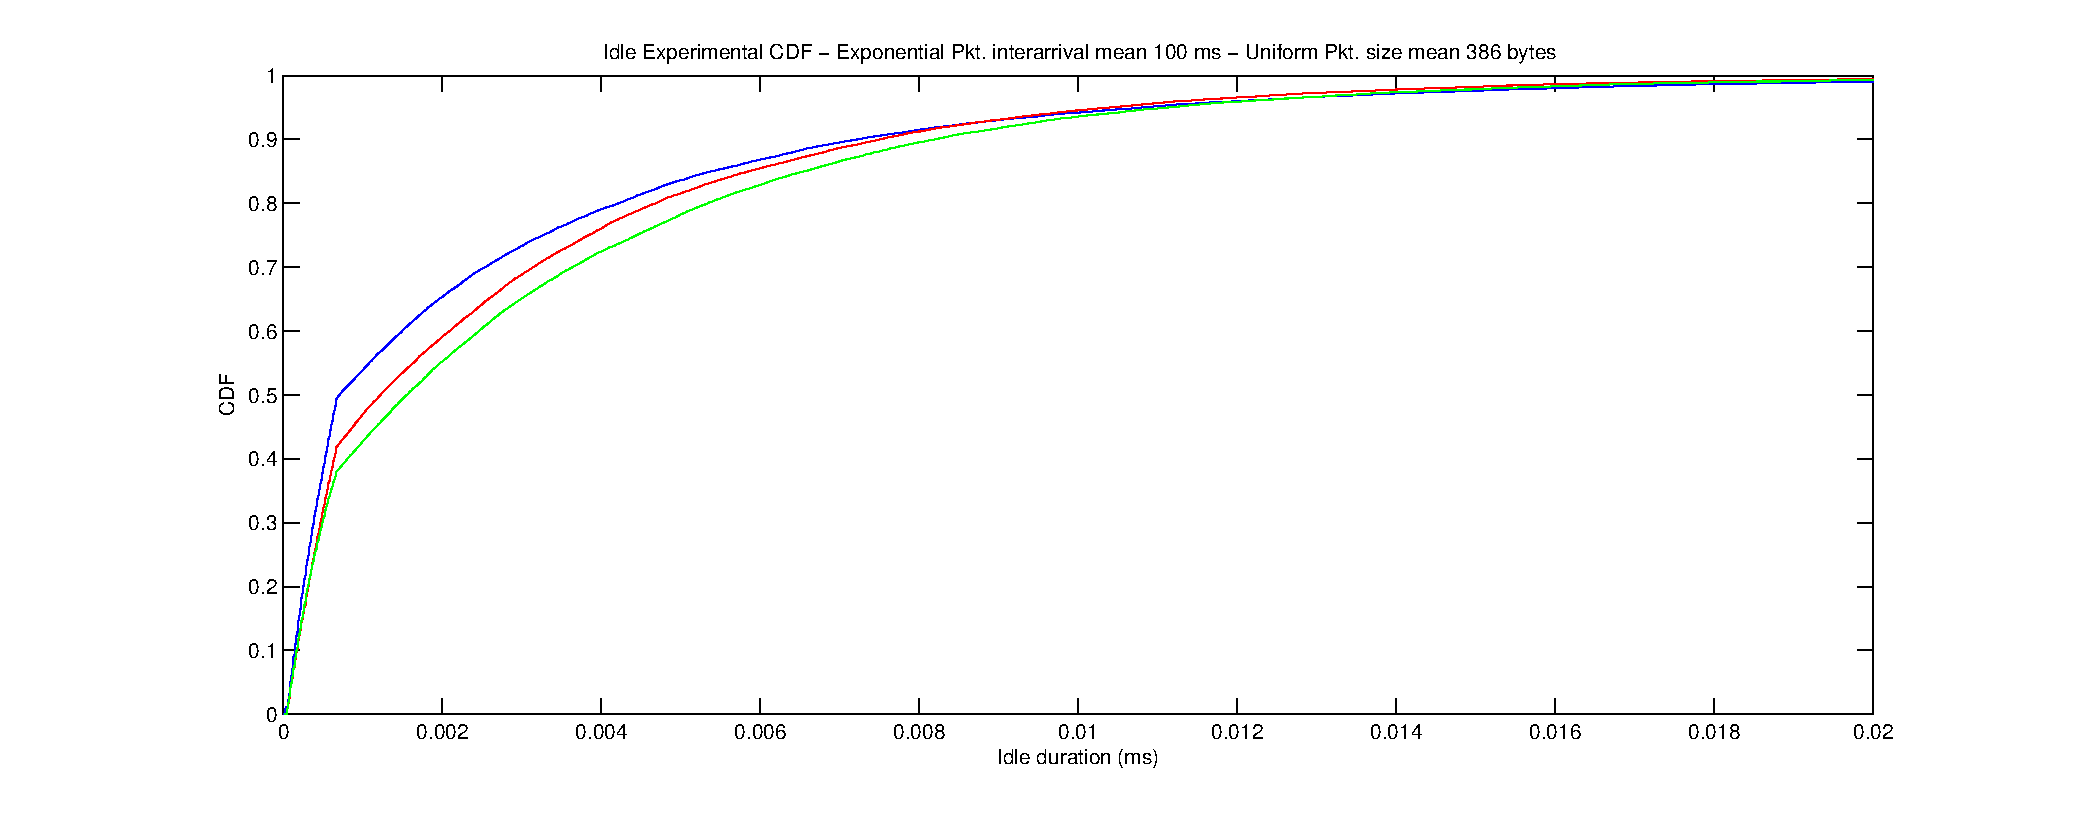
\includegraphics[scale=0.35, trim = 0mm 0mm 6mm 180mm, clip]{images/results/GlobalView/sessions/sessions_composed_cdf}
	\caption{Idle distributions for different number of sessions}
	\label{fig:sessions_composed_cdf}
\end{figure}

As it can be observed in Figure \ref{fig:sessions_composed_cdf}, the mixture model can be used since two differentiated areas can be observed from the Idle distributions: Uniform distribution for $[0 < t < \alpha_{bk}]$ and a long-tail in $[t > \alpha_{bk}]$. Even though, for the high load case, the long-tail behavior is much lower than the other cases meaning that the idle periods will be much shorter than the other two cases.

Since the mixture model can be applied in the three scenarios, it is necessary to check if the estimation process and validation test are being carried properly. For this, we extracted the estimated parameters and the \acs{K-S} values for the 25 runs of each case. It can be observed from Table \ref{table:session_test}, that the variability of the estimated parameters and the \acs{K-S} values can be considered negligible.

\begin{table}[h!]
	\centering
	\begin{tabular}{ c | c | c || c | c || c | c }
		& \multicolumn{2}{ c || }{3 sessions} &  \multicolumn{2}{ c || }{9 sessions} & \multicolumn{2}{ c }{18 sessions}\\ \hline \hline
		& Mean & Std. Deviation & Mean & Std. Deviation & Mean & Std. Deviation \\ \hline
		$\xi$ & 0.110409 & 0.0186127 & 0.115088 & 0.0181082 & 0.0947383 & 0.0168293 \\ 
		$\sigma$ & 0.0110169 & 0.000940108 & 0.00474472 & 2.49E-004 & 0.00307088 & 1.05E-004 \\
		$p$ & 0.135539 & 0.0115675 & 0.337838 & 0.0195118 & 0.535883 & 0.0179058 \\
	\end{tabular}
	\caption{Estimation parameters statistics for different number of sessions}
	\label{table:session_test}
\end{table}

\textcolor{red}{It is necessary to repeat the test with medium-load since the KS failure is higher than the high load case.}

From the \acs{K-S} validation test, we are facing the same behavior as the presented in Section \ref{sec:KS}. For those cases where the ${P<<0.1}$, the deviation between the experimental and empirical distributions is negligible as it is presented in Figure \ref{fig:sessions_ks_fail}. For all the three cases under study in this section, it is possible to reconstruct almost perfectly the empirical distribution from the estimated parameters even the validation test is failing.

% JOHN: Where are the results of the p-value CDF? I could not find them.

\begin{figure}[t]
	\centering
	\includegraphics[scale=0.28]{images/results/GlobalView/sessions/sessions_ks_fail}
	\caption{Fail cases for different number of sessions}
	\label{fig:sessions_ks_fail}
\end{figure}

\subsection{In-session statistics}
The following experiment randomizes what is happening at the flow level. This level describes the behavior of individual sessions, e.g. \acs{WLAN} users. For this experiment the number of sessions will be fixed to a moderate value of traffic load. Following the traffic model defined in \cite{Campus-WLAN}, and the results obtained in this chapter, the different levels of the multi-layer traffic model will be configured as it is presented in Table \ref{tab:sim_traffic_model}.

\begin{table}[htb]
	\begin{center}
		\begin{tabular}{ l | c | c }
			Modeled Variable & Distribution & Parameters \\ \hline
			Session number	& Fixed & 5 users \\
			Session Arrival	 & Fixed & At simulator start \\
			Flow inter-arrival & Log-normal & $\mu = -1.6355$, $\sigma = 2.6286$ \\
			Flow number & Bi-Pareto & $\alpha = 0.07$, $\beta = 1.75$, $c = 295.38$, $k = 1$ \\
			Flow Size & Bi-Pareto & $\alpha = 0.00$, $\beta = 1.02$, $c = 15.56$, $k = 111$ \\
			Packet Size & Uniform & $min = 754$, $max = 2346$ \\
			Packet inter-arrival & Exponential & $\lambda = 10$ \\
		\end{tabular}
		\caption{The parameters used for generating traffic according to the model in \cite{Campus-WLAN}.}
		\label{tab:sim_traffic_model}
	\end{center}
\end{table}

In order to generate a moderate traffic load, the number of sessions (\acs{WLAN} users) has been fixed to 5. Different tests developed with higher number of users had given bad results in the estimation process due to saturation of the network. One of the tests developed with 9 users, following the same configuration defined in Table \ref{tab:sim_traffic_model} and 25 runs had resulted in 80\% of the cases were not estimated (NaN value), since the samples gathered by the sensor were located in the saturated part of the network.

On the other hand, the model presented in Table \ref{tab:sim_traffic_model} will give (with low probability) a high number of flows per session and flow sizes due to the distributions defined and as it can be observed in the results presented in \cite{Campus-WLAN}. One example of our simulations is represented in Figure \ref{fig:high_load_idlecdf}. It can be observed how a high concentration (around 90\%) of the idle periods has a small value, which indicates that the network is saturated. 

\begin{figure}[h!]
	\centering
	\includegraphics[scale=0.28, trim = 0mm 0mm 6mm 180mm, clip]{images/results/GlobalView/flows/high_load/idle_cdf}
	\caption{Idle distribution for high load using traffic model in \ref{tab:sim_traffic_model}}
	\label{fig:high_load_idlecdf}
\end{figure}

500-runs of the simulation with the traffic model presented produced some bad results represented in Figures \ref{fig:high_load_p}, \ref{fig:high_load_nflows}, \ref{fig:high_load_bad_p}. As it can be observed in Figure \ref{fig:high_load_p}, the 60\% of the cases $P<0.1$ which means a high failure rate of the \acs{K-S} test. In addition, results from this test showed some cases where the number of flows per session were higher than 10000 flows and a particular case with 143061 flows. Finally, in order to test if the \acs{K-S} failures still lead to a good fitting between the empirical and estimated distributions, we plotted one case in which the P-value obtained from the validation test is really low. This is represented in Figure \ref{fig:high_load_bad_p}. It can be observed that in this case, not following the behavior presented in Section \ref{sec:KS}, the fitting is not well behaved.

\begin{figure}[h]
	\centering
	\subfloat[]{
		\label{fig:high_load_p}
		\includegraphics[width=0.5\textwidth, trim = 0mm 0mm 0mm 0mm, clip]{images/results/GlobalView/flows/high_load/cdf_p}
	}
	\subfloat[]{
		\label{fig:high_load_nflows}
		\includegraphics[width=0.5\textwidth, trim = 0mm 0mm 0mm 0mm, clip]{images/results/GlobalView/flows/high_load/n_flows}
	}
	\caption{CDF of P-value and flow number using traffic model in \ref{tab:sim_traffic_model}}
\end{figure}

\begin{figure}[h!]
	\centering
	\includegraphics[scale=0.28, trim = 0mm 0mm 0mm 0mm, clip]{images/results/GlobalView/flows/high_load/bad_p}
	\caption{Empirical vs Estimated CDF for low P-value using traffic model in \ref{tab:sim_traffic_model}}
	\label{fig:high_load_bad_p}
\end{figure}

In order to avoid the particular cases in which the number of flows can be triggered to a very high value, the number of flows will be reduced by one order of magnitude (dividing by 10 the number of flows generated by the random distribution). Running again a 500-run simulation we obtained better results for a lower load.

% JOHN: Actually, the conclusion here should twofold: First, we underline the problem with the saturated case: it is not that the fitting fails in the long run; it is more that the time period of network observation is not enough in order to capture a longer-term behavior of the system. So, if we are unlucky to fall inside the saturation period, the estimation fails, and we can not do anything about it.

% Second, we underline that by keeping the distribution shape the same, and only lowering the order of magnitude, solves the problem, that is the estimation does not fail. Either, the fitting is better, or we have more time to gather the samples, right??
 

Figure \ref{fig:limit_cdf_p} show how the \acs{K-S} failure rate is reduced to around 20\% of the cases. On the other hand, the number of flows (Figure \ref{fig:limit_nflows}) generated by the random distribution is reduced and we avoided high number of flows per session, which saturated our network and made the validation test to fail.

\begin{figure}[h]
	\centering
	\subfloat[]{
		\label{fig:limit_cdf_p}
		\includegraphics[width=0.5\textwidth, trim = 0mm 0mm 0mm 0mm, clip]{images/results/GlobalView/flows/limited_load/cdf_p}
	}
	\subfloat[]{
		\label{fig:limit_nflows}
		\includegraphics[width=0.5\textwidth, trim = 0mm 0mm 0mm 0mm, clip]{images/results/GlobalView/flows/limited_load/nflows}
	}
	\caption{CDF of P-value and flow number for reduced traffic model}
\end{figure}

In addition, the number of valid samples for the Idle distribution estimation has been extracted. The number of samples gathered by the sensors for the estimation process during the developed tests in this section are 20000 samples. Figure \ref{fig:limit_samples} show the distribution of the number of valid samples. A sample is considered to be valid for the idle distribution estimation process if $sample > \alpha_{bk}$.

% JOHN: I would also like you to run the tests securing that the samples above the back-off threshold are high enough. Then we put all the results together, here.

\begin{figure}[ht]
	\centering
	\subfloat[]{
		\label{fig:limit_samples}
		\includegraphics[width=0.5\textwidth, trim = 0mm 0mm 0mm 0mm, clip]{images/results/GlobalView/flows/limited_load/samples}
	}
	\subfloat[]{
		\label{fig:limit_load}
		\includegraphics[width=0.5\textwidth, trim = 0mm 0mm 0mm 0mm, clip]{images/results/GlobalView/flows/limited_load/load}
	}
	\caption{CDF of number of valid samples and load in tests where $P-value<0.1$}
\end{figure}

As it can be observed in Figure \ref{fig:limit_samples}, in 50\% of the cases, the number of valid samples is around 6000 or less from the 20000 of the total set of samples, which can be considered a low value for the estimation of the idle distribution.

In order to study what happened in those cases in which the \acs{K-S} test failed, we extracted the load of the network in those cases. The results are presented in Figure \ref{fig:limit_load}. Is interesting how from the cases in which the validation test failed, around 70\% the load was higher than 60\%.

% JOHN: Good. this is a strong point that the problem is, indeed the saturation.

The different results obtained in these set of experiments make us to reconsider the proposed model. The results obtained show that for high loads the estimation failed. On the other hand, the results also show that most of the cases in which the validation test failed for a lower load, the load is higher than 60\%. In order to obtain enough valid samples in cases with moderate-high load the sensor needs to be active for a longer time since most of the samples are in the saturated region of the network affecting the energy-efficiency of the system. One possible approach to modify the model is to avoid the estimation process for those high-load cases improving the energy-efficiency of the sensors.
